\documentclass[border=0.2cm]{standalone}
 
% More defined colors
\usepackage[dvipsnames]{xcolor}
\usepackage{tikz}
\usepackage{xstring}
\usepackage{pgfmath,pgffor}
\usepackage{arrayjob}

\usetikzlibrary{arrows.meta,shapes.arrows, shapes.misc}
\usetikzlibrary{positioning}
\usetikzlibrary{cd, fit, calc}
\usepackage{textcomp}

\begin{document}
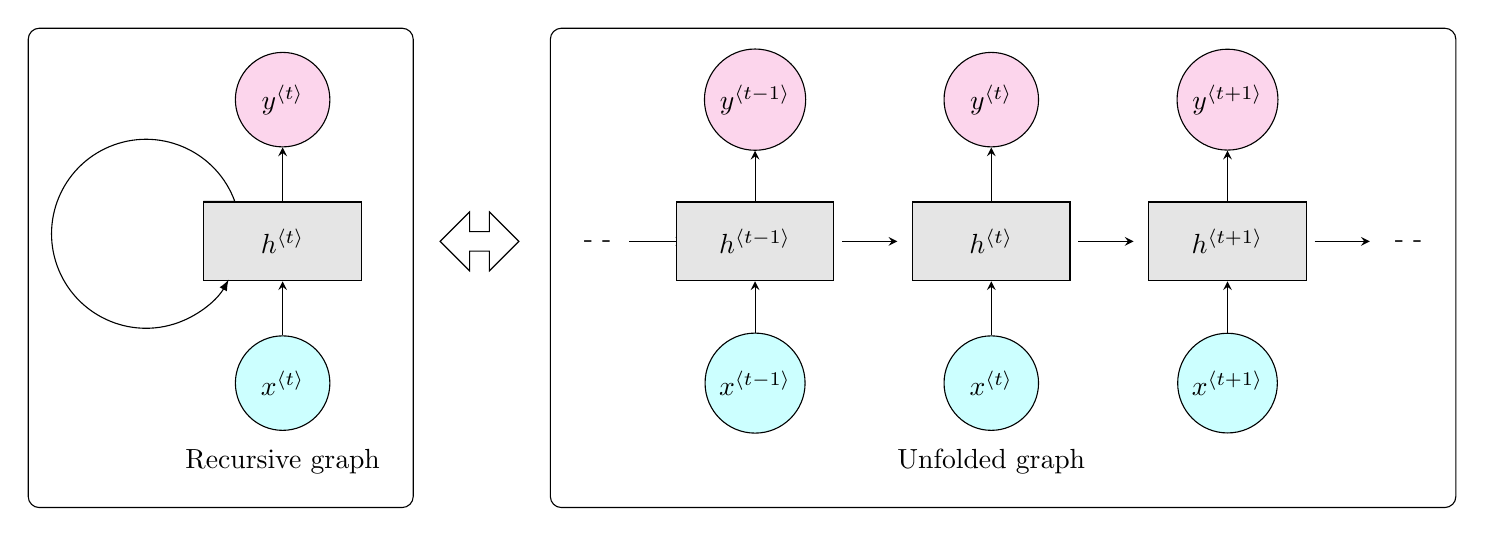
\begin{tikzpicture}

\newcommand{\numlayerA}{3}
\newcommand{\nodedis}{8}

\newarray\indicesarray
\readarray{indicesarray}{-1&&+1}


\node [draw, fill=black!10, minimum width=2cm, minimum height=1cm] (controller1) at (0, 0) {$ h ^{\langle{} t \rangle{} } $ };
\node [draw, circle, minimum size=1.2cm, fill=Rhodamine!20, above of=controller1, node distance=1.8cm ] (circlea1) {$ y ^{\langle{} t \rangle{} } $ };
\node [draw, circle, minimum size=1.2cm, fill=Cyan!20, below of=controller1, node distance=1.8cm ] (circleb1) {$ x ^{\langle{} t \rangle{} } $ };
\draw [stealth-] (circlea1.south) -- (controller1.north) node[midway,right] {};
\draw [-stealth] (circleb1.north) -- (controller1.south) node[midway,right] {};
\draw[-latex] (controller1.north west) -- ++ (.4,0) arc[start angle=20, end angle=331, x radius=1.2cm, y radius =1.2cm] node[midway, right] (feedbackcircle) {};

\node[draw, double arrow, minimum height=10mm, minimum width=.8mm, single arrow head extend=1mm, anchor=west, right of=controller1, node distance=2.5cm] (arrowh) {};

\node[right of=arrowh, node distance=1.5cm] (dot1) {- -};
\draw [-stealth] (dot1.east)+(.1cm,0) -- node[below] (arrow1) {} ++(.8,0);
\node[below of=circleb1, node distance=1cm] (textrecgraph) {Recursive graph};

\node [ rounded corners, draw, inner sep = 3mm, fit={(feedbackcircle) (controller1) (circlea1) (textrecgraph)} ] {};

\foreach \i in {1,...,\numlayerA}
{
    \node [draw, fill=black!10, minimum width=2cm, minimum height=1cm] (controller\i) at (3 + \i*3, 0) {$ h ^{\langle{} t\indicesarray(\i) \rangle{} } $};
    \node [draw, circle, minimum size=1.2cm, fill=Rhodamine!20, above of=controller\i, node distance=1.8cm ] (circlea\i) {$ y ^{\langle{} t\indicesarray(\i) \rangle{} } $ };
    \node [draw, circle, minimum size=1.2cm, fill=Cyan!20, below of=controller\i, node distance=1.8cm ] (circleb\i) { $ x ^{\langle{} t\indicesarray(\i) \rangle{} } $ };
    \draw [stealth-] (circlea\i.south) -- (controller\i.north) node[midway,right] {};
    \draw [-stealth] (circleb\i.north) -- (controller\i.south) node[midway,right] {};
    \draw [-stealth] (controller\i.east)+(.1cm,0) -- node[below] (arrow\i) {} ++(.8,0);
}

\node[below of=circleb2, node distance=1cm] (textunfoldgraph) {Unfolded graph};

\node[right of=controller3, node distance=2.3cm](dot2) {- -}; 
\node [rounded corners, draw, inner sep = 3mm, fit={(dot1) (dot2) (circlea2) (textunfoldgraph)}] {};


\end{tikzpicture}
\end{document}
